\Chapter{数理ファイナンス入門(菊地)}
\Section{\S 1. はじめに}
この記事では,数理ファイナンスという分野を紹介します.
数理ファイナンスというとなんだか数学科らしくないではないか
と思われる方もいらっしゃるかもしれませんが,現在では
数学の中の応用数理の中の分野の一つとして認められています.
%(この記事では全くこだわっていません.)
数理ファイナンスでは,株価などの資産の値動きを
確率的事象として捉えます.
ここでは,主に数理ファイナンスのさきがけとなった
Black-Scholesモデルについて解説します.
この業績でScholesとMerton
\footnote{Mertonは誰かというと,BlackとScholesの議論を
厳密に証明した人です.}
は1997年のノーベル経済学賞を受賞しました.
\footnote{Blackは1995年に亡くなってしまったので
ノーベル賞は受賞していません.}
数学的な用語は最低限に抑えて解説をしたつもりです.
\Section{\S 2. 数理ファイナンスとは}
数理ファイナンスはもともとデリバティブ(金融派生商品)
の価格付けを目的に始まりました.
% 具体的な方法は,株価などの危険資産の値動きを
% 確率的事象として捉え,妥当な仮定のもとで「ある意味」適正な価格をつけます.
% 数学的な用語はできるだけ使わないで解説をします.
\Subsubsection{基本的な用語}
\begin{itemize}
 \item 危険資産:株式や債券などの不確実な出来事の影響で価格が
       決まる資産のこと.
 \item 安全資産:銀行預金のように確実な資産.
 \item デリバティブ\footnote{実はデリバティブの考え方は自然なものです.
       例えば,
       http://www.shiruporuto.jp/finance/kinyu/deriv/に起源などに関する
       説明が載ってます.}
       :株式や債券,農産物や鉱石などを原資産とする派生商品.
 \item ポートフォリオ:投資家が保有している資産の組み合わせのこと.
       たとえば,A社の株式$a$単位,銀行預金$b$など.
\end{itemize}
\kikueg ヨーロピアンオプション\\
ヨーロピアンオプションは2つのパラメータ満期日$T$と行使価格$K$
によって特徴づけられます.満期日$T$,行使価格$K$のヨーロピアンコールオプションと
は,満期日$T$(現在時刻は$t=0$とします.)にある危険資産$1$単位を
行使価格$K$で購入できる権利のことを言います.
(権利なので,満期日に買わなくてはならないというわけではありません.)
また,逆に満期日$T$に行使価格$K$である危険資産を$1$単位売ることができる
権利のことをヨーロピアンプットオプションといいます.
他にも,満期日以前のどのタイミングでも権利を行使できる
アメリカンオプションなどデリバティブの種類はかなりたくさんありますが,
今回はヨーロピアンコールオプションの適切な価格付けを考えます.
まずは,ヨーロピアンコールオプションのペイオフ(購入者への支払い)
について考えておきましょう.\\
時刻$t(0\leq t\leq T)$における原資産の価格を$S(t)$とします.
合理的なヨーロピアンコールオプションの購入者は,
\[
\begin{cases}
 S(t)>K\Longrightarrow 権利行使\\
 S(t)\leq K\Longrightarrow 権利破棄
\end{cases}
\]
となるように行動します.
したがって,ペイオフは$(S(t)-K)^+$となります.
ただし,$(S(t)-K)^+=\max\{S(t)-K,\ 0\}$とします.
グラフは次のようになります.
\[
\input{kikuchicall.tpc}
\]
\Subsubsection{基本的な仮定}
数学的なモデルを作るにあたって,以下のような仮定をします.
\begin{itemize}
 \item 株式に配当はない.
 \item 任意の時刻で危険資産に価格が付いており,その価格で
       任意の実数単位での売買が可能.
 \item 空売り(保有していない資産を他者から借りてきて売る行為.
       当然,借りた資産は将来の適当な時点で返却しなければならない.)
       も可能.
 \item 任意の時刻で任意の実数金額の銀行預金,借り入れが可能.
 \item 預金金利と借り入れ金利は等しい.
 \item 手数料や税金は一切なし.
\end{itemize}
他にも,現実の世界との差を書くべきところがあるかもしれませんが,
以降は理想的な市場であると考えてください.
\Section{\S 3. 価格づけとは?}
%\label{whatsprice}
ここでは,1期間二項モデルと呼ばれる単純なモデルで
価格付けはどのようにして行われるべきかを考えます.
\\
ある株式を原資産とする満期日$T=1$,行使価格$K=125$の
ヨーロピアンコールオプションについて考えます.
二項モデルでは,時間は離散的なもの($t=1,2,3,\ldots$)
として,各時点において株価は次の時点に移るときに
2つの可能性のみを考えます.
ここでは,原資産である株式の値動きは次のようになるとします.
また,金利は$r=0.25$とします.
\[
 \input{kikuchibinomial.tpc}
\] 
この場合のペイオフは
\[
 \begin{cases}
  S(1)=200\Longrightarrow 75\\
  S(1)=50\Longrightarrow 0
 \end{cases}
\]
となります.このとき,次の投資戦略を考えます.\\
\\
$t=0$:
\begin{center}
 \begin{tabular}{|l|c|c|}\hline
  & 現金&株式保有数 \\ \hline \hline
  初期保有&30 &0 \\
  銀行から20借り&+20 &$\pm$ 0 \\
  株式0.5単位買い&$-50$ &+0.5 \\ \hline
  &0 &0.5 \\ \hline
 \end{tabular}
\end{center}
% \newpage
$t=1$:
\begin{table}[htbp]
  \begin{center}
    \begin{tabular}{c}

      % 1
      \begin{minipage}{0.5\hsize}
        \begin{center}
          \begin{tabular}{|l|c|c|}
            \hline
            $S(1)=200$のとき & 現金 & 株式 \\ \hline \hline
            $t=0$での保有 & 0 & $0.5$ \\
            株式$0.5$単位売り & $+100$ & $-0.5$ \\
            銀行に$25$返す & $-25$ & $\pm$0 \\ \hline
             & 75 & 0 \\
            \hline
          \end{tabular}
        \end{center}
      \end{minipage}

      % 2
      \begin{minipage}{0.5\hsize}
        \begin{center}
          \begin{tabular}{|l|c|c|}
            \hline
            $S(1)=50$のとき & 現金 & 株式 \\ \hline \hline
            $t=0$での保有 & 0 & $0.5$ \\
            株式$0.5$単位売り & $+25$ & $-0.5$ \\
            銀行に$25$返す & $-25$ & $\pm$0 \\ \hline
             & 0 & 0 \\
            \hline
          \end{tabular}
        \end{center}
      \end{minipage}

    \end{tabular}
  \end{center}
\end{table}
\\
\\
この投資戦略のペイオフはヨーロピアンコールオプションと一致しています.
このとき,この投資戦略はヨーロピアンコールオプションを複製する
と言います.
この複製にかかった費用は初期費用の$30$だけです.
このとき,ヨーロピアンコールオプションの価格は$30$になることが
次のような経済学的な議論によって確認できます.
\\
実際,価格が$30$よりも高いとすると,ヨーロピアンコールオプション
を売って,上と同じ投資戦略を,
$30$よりも低い場合は,ヨーロピアンコールオプションを買って,
上と逆の投資戦略を取ると,
それぞれ$30$との差額分の利益が確実に得られる.
(これを裁定機会という.)
このように複製費用と市場価格の間に乖離があるとすれば,
市場の人たちはみな裁定機会を用いて利益をあげようとするので,
需要と供給の関係によって,
価格が$30$よりも高い場合は,価格が下がり,
$30$よりも低い場合は価格が上がる.
また,均衡価格は$30$である.
\\
このように経済学的に妥当な議論を加えることによって,
適正な価格付けを以下のように定めることができます.
\footnote{実際にはデリバティブがいつでも複製可能とは限りません.
また,複製の方法もひと通りとは限りません.}
\begin{screen}
 デリバティブの市場価格は複製費用と一致する.
 また,この価格のことを裁定価格という.
\end{screen}
以下,価格付けと言ったら,裁定価格を求めることを指すことにし,
裁定価格は複製費用であるとします.
\Section{\S 4. 確率論からの準備}
%\ref{whatsprice}
前節では二項モデルを用いて適正価格とはなにか
を考えました.
しかし,二項モデルはあまりにも現実世界との乖離が大きいです.
したがって,これからは時間を連続(時間を実数にして考えるということです.)
にとって考えることを考えます.
\footnote{もちろん,現実世界でも連続的に取引は行われているわけではありませんが,最近ではミリ秒単位で売買を繰り返す
HFT(High Frequency Trade)が主流になっているようなので,
近似として連続時間を考えることはそれほど的外れではありません.}
\Subsubsection{ブラウン運動}
連続時間でランダムな動きを記述する最もスタンダードな方法は
次にあげるブラウン運動を用いる方法です.
\\
%\begin{screen}
 ブラウン運動$W(t)$とは,以下を満たすものです.
 \footnote{数学的に厳密な定義ではありません.}
\begin{enumerate}
\renewcommand{\labelenumi}{\roman{enumi})}
 \item $W(0)=0$.
 \item $0=t_0<t_1<\cdots<t_n=T$に対して,
       各増分$W(t_{i+1})-W(t)$は互いに独立で平均$0$,分散$t_{i+1}-t_i$
       の正規分布に従う.
\end{enumerate}
%\end{screen}
たとえば,ブラウン運動は次のような道を持ちます.
\[
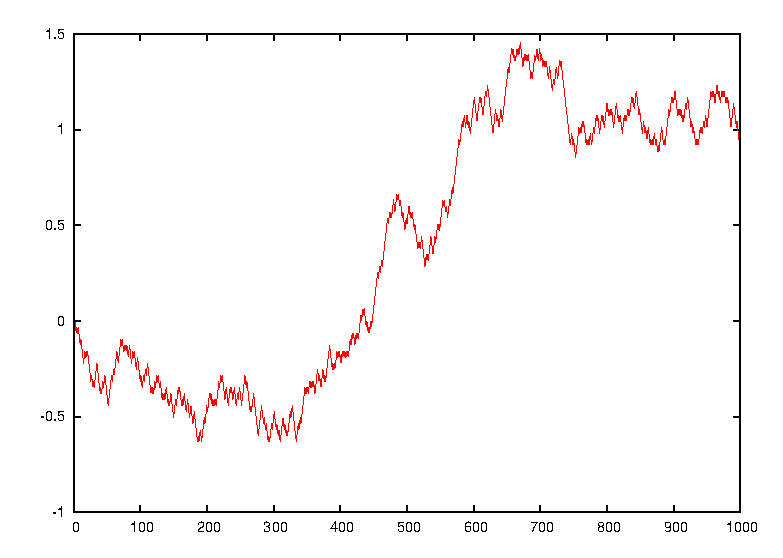
\includegraphics[width=10cm]{kikuchiBM_2.eps}
\]
\Subsubsection{確率積分}
確率積分とはブラウン運動に沿った積分のことです.
つまり,被積分関数と微小時間におけるブラウン運動の差分
をかけあわせたものを足しあげたものが確率積分です.
\footnote{これはざっくりとした説明です.数学的に厳密に
確率積分を構成するには確率論の知識が必要です.}
これは数理ファイナンスで言うと,ある時刻から他の時刻までの
利益を計算するときに使います.
確率積分は次のように書かれます.
\begin{equation*}
 X=\int_{0}^{T}f(t)dW(t).
\end{equation*}
また,これは直感的な理解がしやすいように微分形で書かれることもあります.
\begin{equation*}
 dX=fdW.
\end{equation*}
\Subsubsection{伊藤の公式と伊藤過程}
次は伊藤の公式と呼ばれているもので,通常の微積分で言うと
合成関数の微分公式にあたります.
\[
 df(t,W(t))=\frac{\D f}{\D t}dt+\frac{\D f}{\D x}dW+
 \frac{1}{2}\frac{\D^2f}{\D x^2}dt.
\]
これは,形式的に左辺をTaylor展開することによって,次のような
規則であると考えることもできます.
\begin{screen}
\begin{center}
 $dWdW=dt,\ dtdW=dWdt=0,\ dtdt=0.$
\end{center}
\end{screen}
また,次のような形を持つものを伊藤過程と言います.
\[
 dX(t)=\Delta (t)dW(t)+\theta (t)dt.
\]
伊藤過程についての積分を次のように定義します.
\[
 \int_{0}^{T}\Gamma (t)dX(t)=\int_{0}^{T}\Gamma(t)\Delta(t)dW(t)
 +\int_{0}^{T}\Gamma(t)\theta(t)dt.
\]
伊藤過程についても伊藤の公式が成り立ちます.
\begin{eqnarray*}
 df& = &\frac{\D f}{\D t}dt+\frac{\D f}{\D x}dX
 +\frac{1}{2}\frac{\D^2f}{\D t^2}dtdt+\frac{\D^2f}{\D t\D x}dtdX
 +\frac{1}{2}\frac{\D^2f}{\D x^2}dXdX\\
 & = &\frac{\D f}{\D t}dt+\frac{\D f}{\D x}\Delta dW 
 +\frac{\D f}{\D x}\theta dt+
 \frac{1}{2}\frac{\D^2 f}{\D x^2}\Delta^2dt.\\ 
\end{eqnarray*}
\kikueg 幾何ブラウン運動
\\
定数$\alpha$と$\sigma$に対して,
\[
 X(t)=\int_{0}^{t}\sigma dW(s)+
 \int_{0}^{t}\left(\alpha-\frac{1}{2}\sigma^2\right)ds
\]
とおきます.
また,定数$S(0)$と$f(x)=S(0)\exp x$に対して
\[
 S(t)=f(X(t))
\]
を幾何ブラウン運動と言います.
実は,幾何ブラウン運動は1期間二項モデルを多期間にして,
極限を取ると現れます.
\\
伊藤の公式によって次が成り立ちます.
\begin{eqnarray*}
 dS(t)& = &df(X(t))\\
 & = &\frac{\D f}{\D x}dX(t)+\frac{1}{2}\frac{\D^2f}{\D x^2}dXdX \\
 & = &S(t)dX(t)+\frac{1}{2}S(t)\sigma^2dt \\
 & = &\alpha S(t)dt+\sigma S(t)dW(t).
\end{eqnarray*}
\Section{\S 5. Black-Scholesモデル}
それではファイナンスの話題に戻りましょう.
ここでは最もスタンダードなBlack-Scholesモデルを考えます.
このモデルは,1種類の株式と1種類の銀行預金が存在する市場について
分析します.
$S(t)$を時刻$t$での株価とします.ここでは,$S(t)$は幾何ブラウン運動
に従うものとします.
\[
 dS(t)=\alpha S(t)dt+\sigma S(t)dW(t).
\]
また,金利は$r>0$とします.
次に,$X(t)$を時刻$t$でのポートフォリオの価値とします.
すると,$X(t)$は次の確率微分方程式を満たします.
\[
 dX(t)=\Delta(t)dS(t)+r(X(t)-\Delta(t)S(t))dt.
\]
ただし,$\Delta(t)$は時刻$t$での株式保有数とします.
この式は,右辺の第1項が株式への投資額,第2項が銀行預金の額
の微小時間における差分を表しています.
$dS(t)$に幾何ブラウン運動を代入して計算を進めると,
\[
 dX(t)=rX(t)dt+\Delta(t)(\alpha-r)S(t)dt+\Delta(t)\sigma S(t)dW(t)
\]
となります.
ここで,$c(t,x)$を時刻$t$,株価$x$でのヨーロピアンコールオプションの
価格とします.
すると,伊藤の公式より,
\begin{eqnarray*}
 dc(t,S(t))& = &\frac{\D c}{\D t}dt+\frac{\D c}{\D x}dS+
  \frac{1}{2}\frac{\D^2c}{\D x^2}dSdS\\
 & = &\frac{\D c}{\D t}dt+
  \frac{\D c}{\D x}\left(\alpha S(t)dt+\sigma S(t)dW(t)\right)+
  \frac{1}{2}\sigma^2S^2\frac{\D^2c}{\D x^2}dt\\
 & = &\left(\frac{\D c}{\D t}+\alpha S(t)\frac{\D c}{\D x}+
  \frac{1}{2}\sigma^2S^2\frac{\D^2c}{\D x^2}\right)dt+
  \sigma S\frac{\D c}{\D x}dW
\end{eqnarray*}
となります.
したがって,ポートフォリオ$X(t)$でヨーロピアンコールオプションを
複製するためには,
\[
 X(0)=c(0,S(0)),\ dX(t)=dc(t,S(t))
\]
となれば良いので,$dW$の項を比較して
\[
 \Delta(t)=\frac{\D c}{\D x}(t,S(t)),
\]
$dt$の項を比較して,
\begin{eqnarray*}
 rX(t)& = &rc(t,S(t)) \\
 & = &\frac{\D c}{\D t}(t,S(t))+rS(t)\frac{\D c}{\D x}(t,S(t))+
  \frac{1}{2}\sigma^2S^2(t)\frac{\D^2c}{\D x^2}(t,S(t))
\end{eqnarray*}
となります.最初の式は,株式保有数は右辺のようにすればよい
ということを示しています.これはデルタヘッジと呼ばれます.
また,第2式から
\[
 rc(t,x)=\frac{\D c}{\D t}(t,x)+rx\frac{\D c}{\D x}(t,x)+
  \frac{1}{2}\sigma^2x^2\frac{\D^2c}{\D x^2}(t,x)
\]
と適当な境界条件
を満たす$c(t,x)$を見つければ良いことが分かります.
この偏微分方程式をBlack-Scholes方程式と言います.
\Section{\S 6. BS方程式を解く}
では,最後にBlack-Scholes方程式を解きましょう.
まずは,$y=\log x$と変数変換します.すると,
\begin{eqnarray*}
 \frac{\D}{\D x}& = &\frac{1}{x}\frac{\D}{\D y},\\
 \frac{\D^2}{\D x^2}& = &-\frac{1}{x^2}\frac{\D}{\D y}+\frac{1}{x^2}
  \frac{\D^2}{\D y^2}
\end{eqnarray*}
となります.また,$\tau = T - t$とすると,
\[
 \frac{\D}{\D t}=-\frac{\D}{\D\tau}
\]
となります.これらの変数変換によってBlack-Scholes方程式は
次のように変形できます.
\[
 -\frac{\D c}{\D\tau}+\left(r-\frac{1}{2}\sigma^2\right)
 \frac{\D c}{\D y}+\frac{1}{2}\sigma^2\frac{\D^2c}{\D y^2}-rc=0.
\]
次に,
\[
\begin{cases}
 \alpha=\frac{1}{2}-\frac{r}{\sigma^2}\\
 \beta=-\frac{1}{8\sigma^2}(\sigma^2+2r)^2
\end{cases}
\]
に対して,$c=\exp(\alpha y+\beta\tau)U$
とすると,
\[
 -\frac{\D U}{\D\tau}+\frac{1}{2}\sigma^2\frac{\D^2U}{\D y^2}=0
\]
となります.
ここで,$\tau$を改めて$\frac{1}{2}\tau\sigma^2$とすると,
\[
 \frac{\D U}{\D\tau}=\frac{\D^2U}{\D y^2}
\]
となります.
これは,熱伝導を記述する熱方程式というものになっています.
このように変形して数値計算すると,$c(t,x)$は次のような形になることが
分かります.\footnote{Black-Scholes方程式は解析解を持ちますが,
長くなるのでここでは省略します.}
ただし,実線はペイオフを表し,点が数値計算により
得られたヨーロピアンコールオプションの価格を示しています.
\[
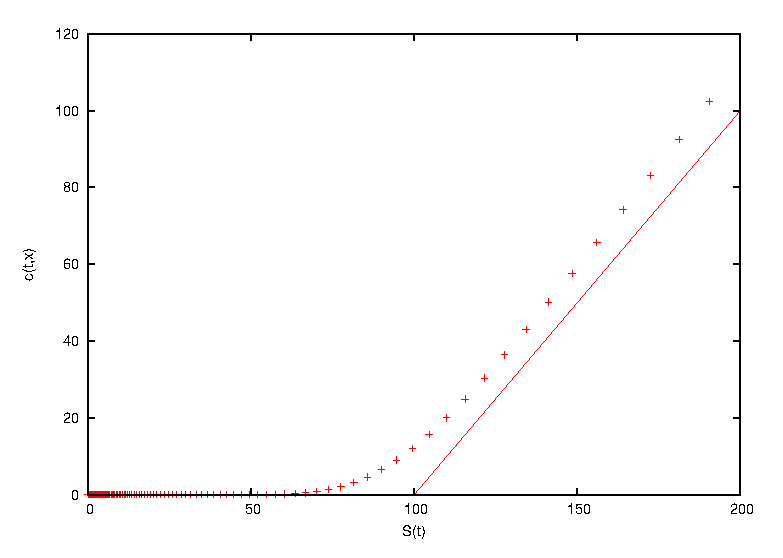
\includegraphics[width = 10cm]{kikuchiBS.eps}
\]
%\begin{thebibliography}{9}
% \bibitem
% \bibitem 
%\end{thebibliography}

\Section{参考文献}
\begin{description}
\item{[1]} Steven E. Shreve,``Stochastic Caluculus for Finance II  Continuous-Time Models'',Springer
\item{[2]} 関根順,``数理ファイナンス'',培風館
\end{description}
